
\subsection{ Open WebUI -  web interface for LLM chat}\

Run\textbf{ Open WebUI} via Docker, and be sure to use the\textbf{ CUDA‑enabled} version because it needs to run on the\textbf{ GPU}.

Note:
\begin{enumerate}
    \item The\textbf{ CUDA} version is required.
    \item The external default service port is \textbf{3000}, but it can be changed.
    \item he container service starts and stops \textbf{automatically} in sync with the server’s startup and shutdown.
    \item If pulling the Docker image fails or is slow, switch to a different\textbf{ image mirror} or use a \textbf{VPN}.
\end{enumerate}

\vspace{0.5cm}

\begin{lstlisting}
docker run -d -p 3000:8080 --gpus all --add-host=host.docker.internal:host-gateway -v open-webui:/app/backend/data --name open-webui --restart always ghcr.io/open-webui/open-webui:cuda
\end{lstlisting}

Login to Open Webui at \textbf{http://172.16.33.244:3000} . When you log in for the first time, you need to create a \textbf{administrator account} and password. Subsequent users can register themselves, and the system will \textbf{automatically approve} the registrations (you can optionally configure the approval to require a administrator’s confirmation instead). Currently, the admin user name is : \textbf{q30china@gmail.com}, password:\textbf{ hexing@2025}

\begin{figure}[H]
    \begin{center}
        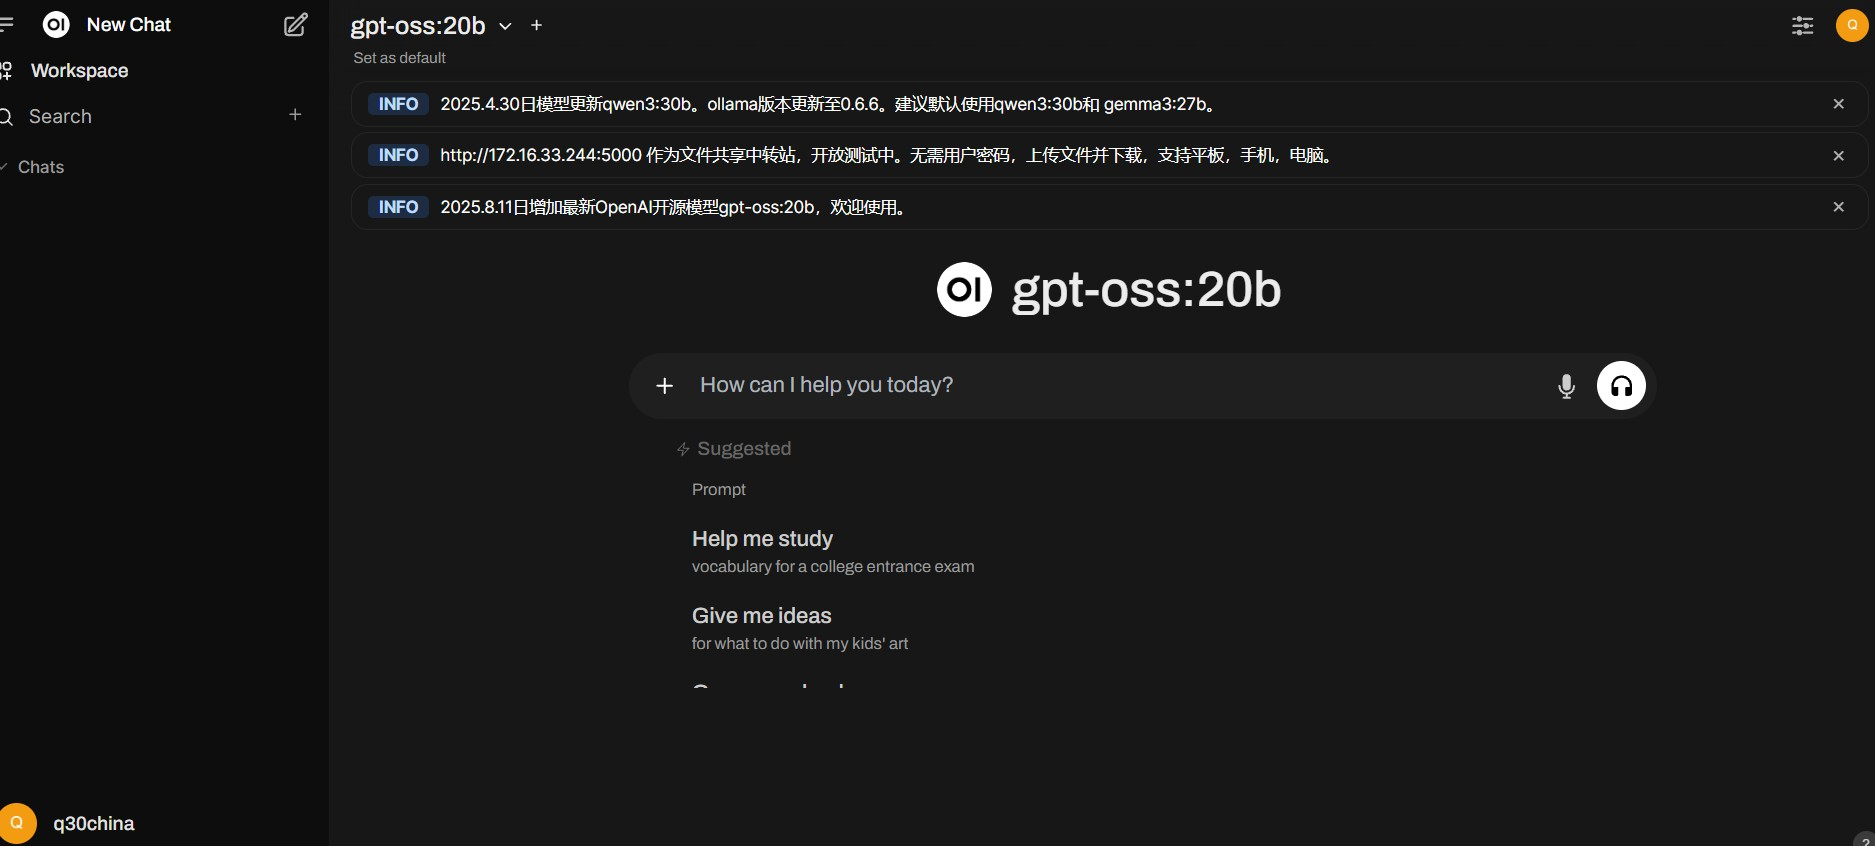
\includegraphics[width=.95\linewidth]{res/open-webui.jpg}\\
        \caption{Open Webui User Interface }\label{open-webui}
    \end{center}
\end{figure} 

\subsection{ Ragflow - Retrieval‑Augmented Generation (RAG) systems}\

Run all the container images with Docker. Once they start normally, the service will be exposed on the default port 8080 . During the first initialization you must set up a system‑administrator account and password. Currently, the admin user name is : \textbf{q30china@gmail.com}, password:\textbf{ hexing@2025}

\vspace{0.5cm}

\begin{lstlisting}
# start the service
cd /data/git/ragflow/docker
docker compose -f docker-compose-gpu.yml up -d

# stop the service
docker compose -f docker-compose-gpu.yml down
\end{lstlisting}

\vspace{0.5cm}

\begin{figure}[H]
    \begin{center}
        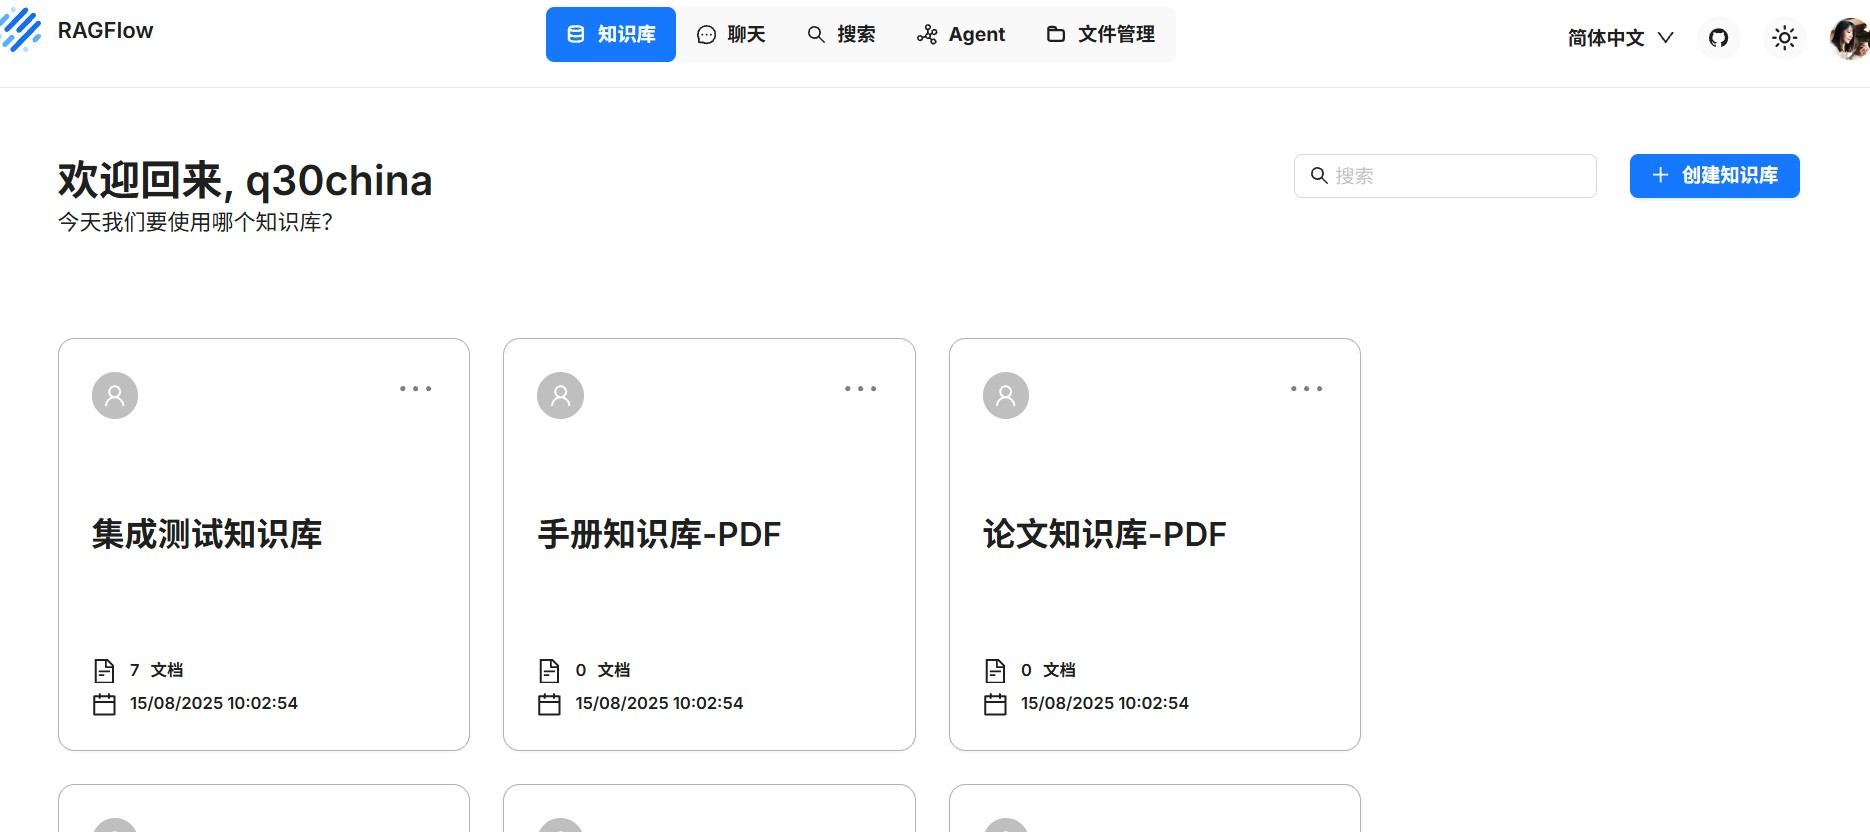
\includegraphics[width=.95\linewidth]{res/ragflow.jpg}\\
        \caption{Ragflow User Interface }\label{ragflow}
    \end{center}
\end{figure} 

How to use the Ragflow local knowledge database, and create a web application to use this.

step 1: Add local models service (Ollama is running)

\begin{figure}[H]
    \begin{center}
        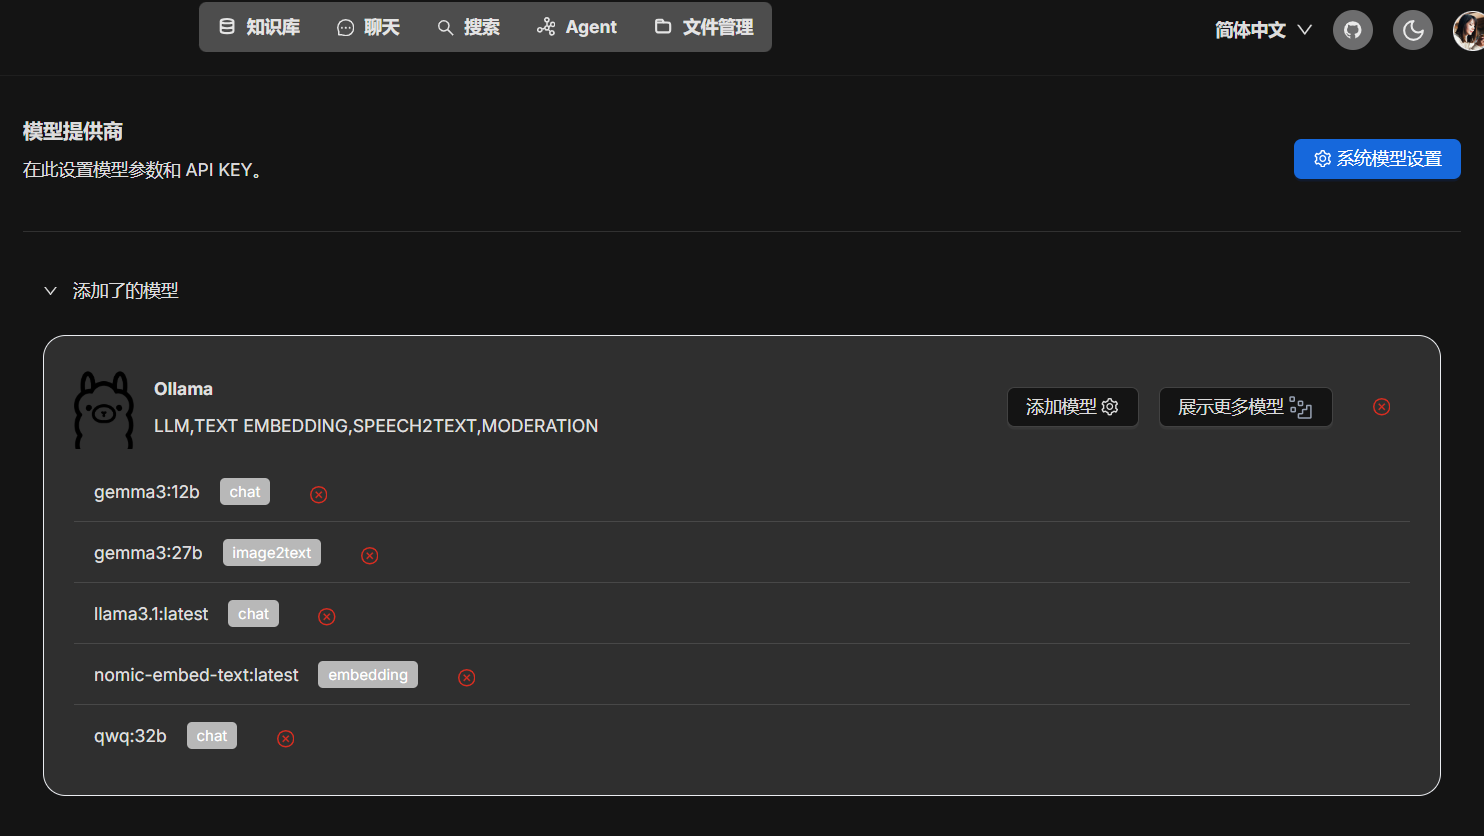
\includegraphics[width=.95\linewidth]{res/ragflow-addmodel.png}\\
        \caption{Add local models }\label{ragflow-addmodel}
    \end{center}
\end{figure}

step 2: Create a new knowledge base, upload local documents, and wait until the system has finished parsing and vectorizing the storage before proceeding.

\begin{figure}[H]
    \begin{center}
        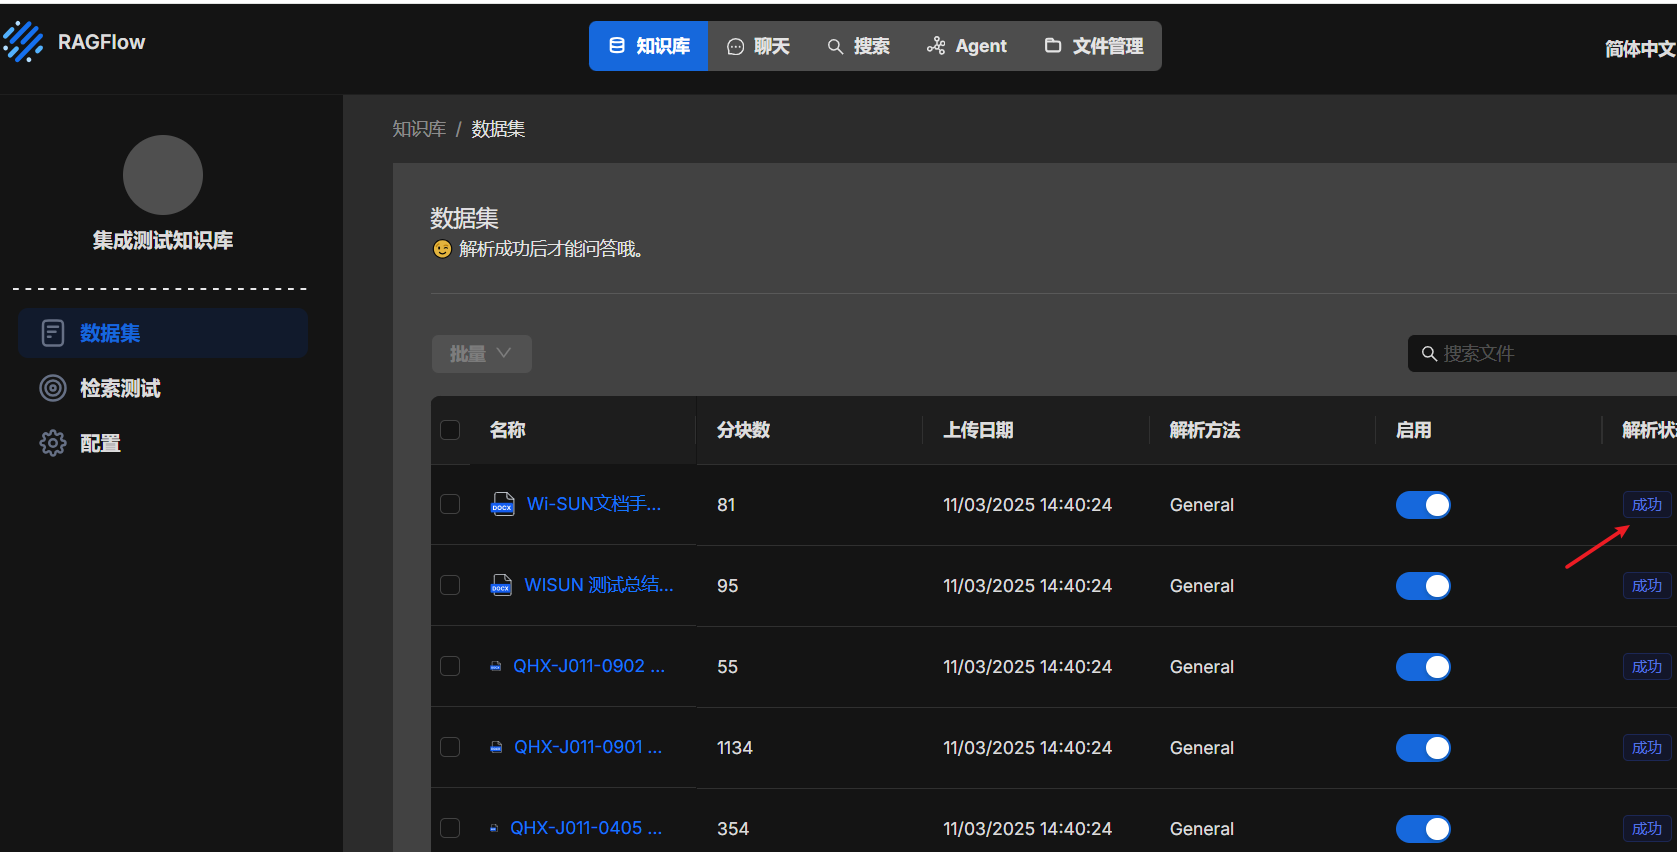
\includegraphics[width=.95\linewidth]{res/ragflow-upload.png}\\
        \caption{Upload local files to knowledge database }\label{ragflow-upload}
    \end{center}
\end{figure}

step 3: In the knowledge‑base configuration screen, be sure to select the document’s language and choose the embedded vector model (pulled via Ollama). Adjust any other parameters as needed, but typically the defaults are fine.

\begin{figure}[H]
    \begin{center}
        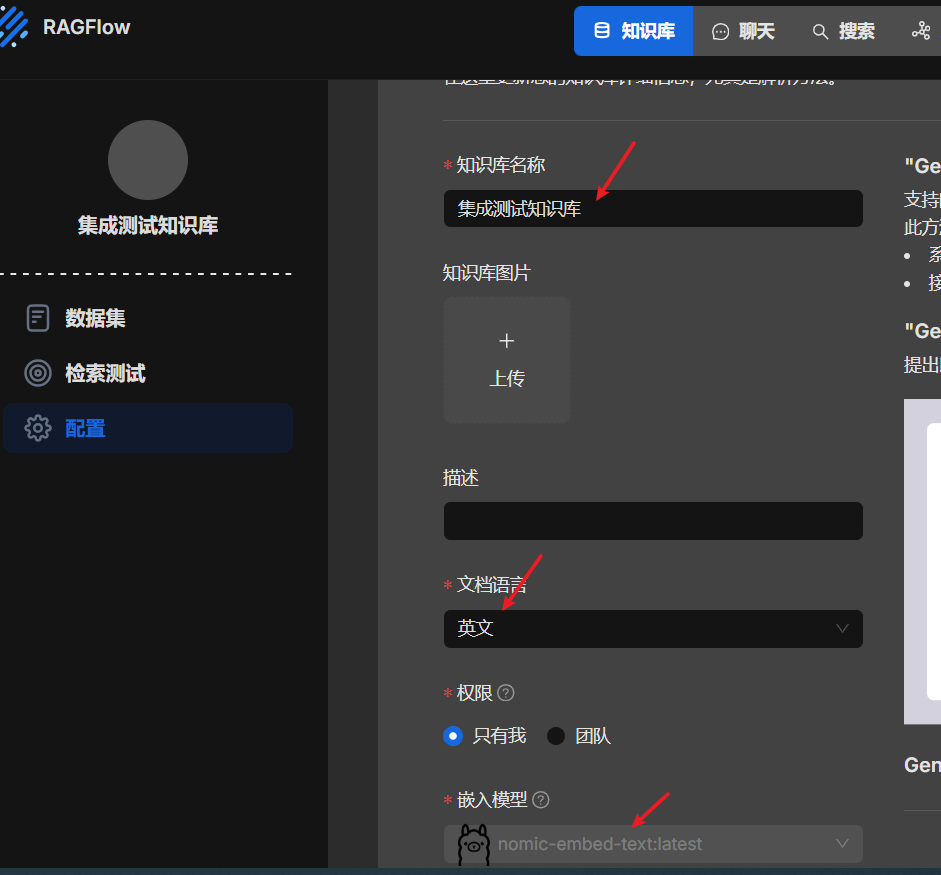
\includegraphics[width=.95\linewidth]{res/ragflow-embeded.png}\\
        \caption{Configuration of knowlege database }\label{ragflow-embeded}
    \end{center}
\end{figure}

step 4: Create a new digital‑human application for new‑employee training, using the locally created knowledge base and configuring the LLM to a model from the local Ollama service.

\begin{figure}[H]
    \begin{center}
        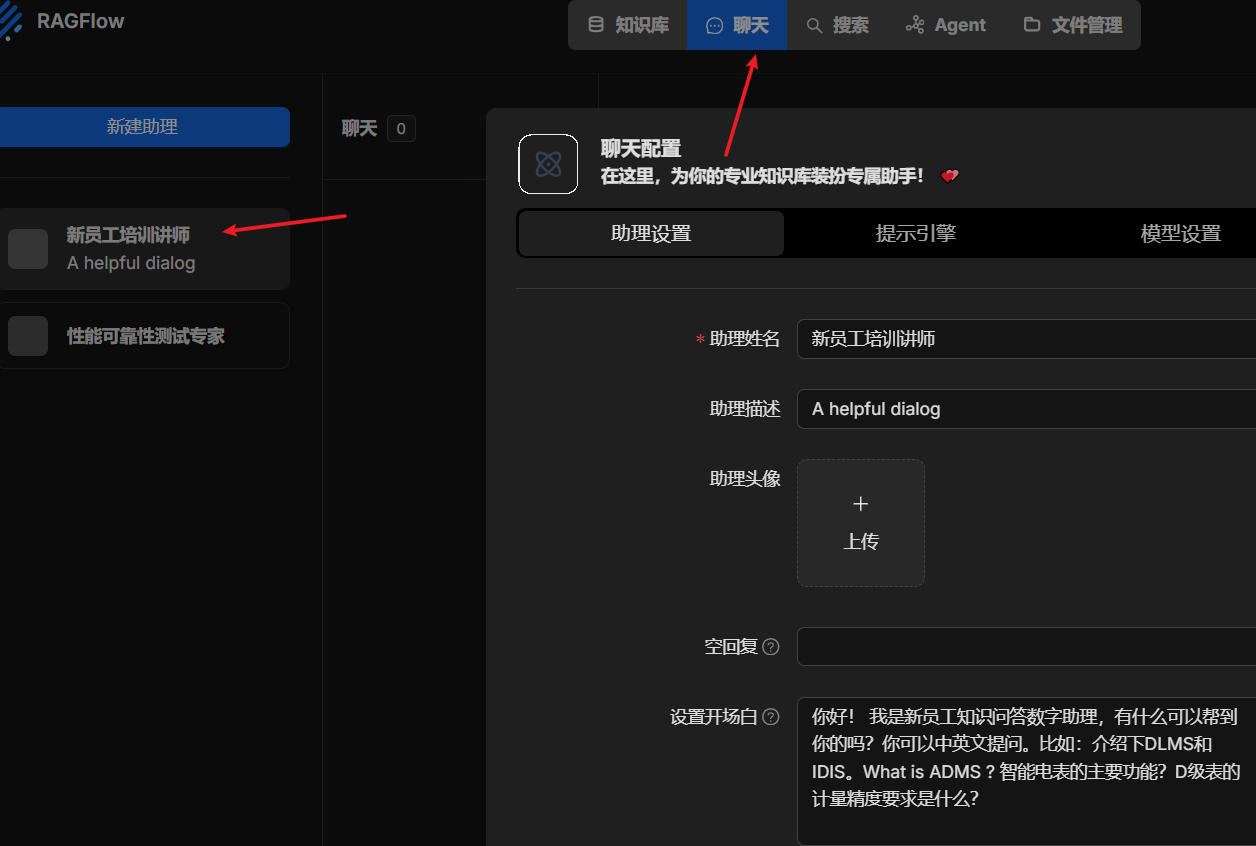
\includegraphics[width=.95\linewidth]{res/ragflow-app.png}\\
        \caption{Create application }\label{ragflow-app}
    \end{center}
\end{figure}

step 5: Publish app, and test, also can embedded the link to your own web.

\begin{minted}[frame=single,framesep=1mm,breaklines=true]{html}
<iframe
src="http://172.16.33.244:8080/chat/share?shared_id=da54fcfe
f9a311efa8a70242ac120006&from=chat&auth=
FiYWQ3MzMwZjgxMzExZWZhNmZlMDI0Mm"
style="width: 100%; height: 100%; min-height: 600px"
frameborder="0"
>
</iframe>
\end{minted}

\begin{figure}[H]
    \begin{center}
        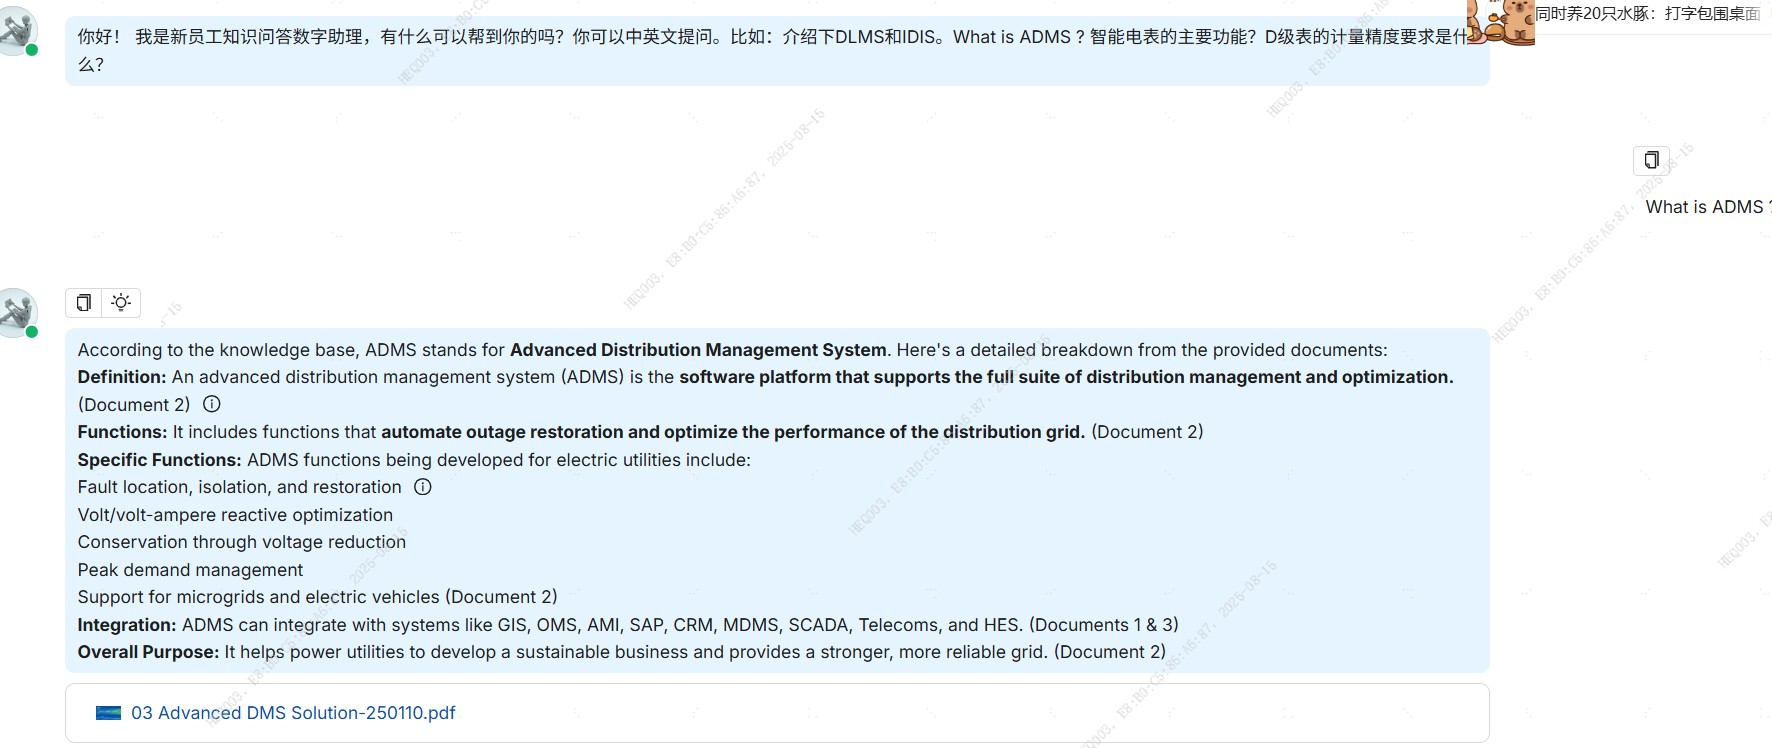
\includegraphics[width=.95\linewidth]{res/ragflow_qa.jpg}\\
        \caption{Test the Digital Human }\label{ragflow_qa}
    \end{center}
\end{figure}

